\documentclass{standalone}
\usepackage{tikz}

\begin{document}
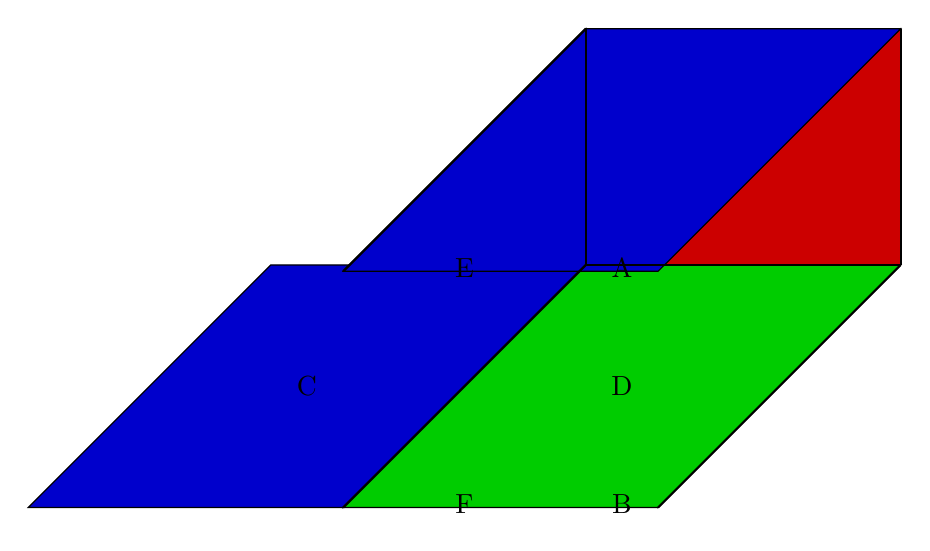
\begin{tikzpicture}[scale=2]

% Define colors for the prism
\definecolor{basecolor1}{RGB}{255, 0, 0} % Red
\definecolor{basecolor2}{RGB}{0, 255, 0} % Green
\definecolor{basecolor3}{RGB}{0, 0, 255} % Blue

% Define the coordinates of the prism
\def\prismheight{4}
\def\prismwidth{2}
\def\prismdepth{1.5}

% Draw the prism
\filldraw[fill=basecolor1!80!black, draw=black] (0,0,0) -- ++(\prismwidth,0,0) -- ++(0,\prismdepth,0) -- ++(-\prismwidth,0,0) -- cycle;
\filldraw[fill=basecolor2!80!black, draw=black] (0,0,0) -- ++(0,\prismdepth,0) -- ++(0,0,\prismheight) -- ++(0,-\prismdepth,0) -- cycle;
\filldraw[fill=basecolor3!80!black, draw=black] (0,0,0) -- ++(0,0,\prismheight) -- ++(-\prismwidth,0,0) -- ++(0,0,-\prismheight) -- cycle;
\filldraw[fill=basecolor1!80!black, draw=black] (\prismwidth,0,0) -- ++(0,\prismdepth,0) -- ++(0,0,\prismheight) -- ++(0,-\prismdepth,0) -- cycle;
\filldraw[fill=basecolor2!80!black, draw=black] (\prismwidth,0,0) -- ++(0,0,\prismheight) -- ++(-\prismwidth,0,0) -- ++(0,0,-\prismheight) -- cycle;
\filldraw[fill=basecolor3!80!black, draw=black] (0,\prismdepth,0) -- ++(0,0,\prismheight) -- ++(\prismwidth,0,0) -- ++(0,0,-\prismheight) -- cycle;

% Draw the edges of the prism
\draw[thick, black] (0,0,0) -- ++(\prismwidth,0,0);
\draw[thick, black] (0,0,0) -- ++(0,\prismdepth,0);
\draw[thick, black] (0,0,0) -- ++(0,0,\prismheight);
\draw[thick, black] (\prismwidth,0,0) -- ++(0,\prismdepth,0);
\draw[thick, black] (\prismwidth,0,0) -- ++(0,0,\prismheight);
\draw[thick, black] (0,\prismdepth,0) -- ++(0,0,\prismheight);

% Add letter labels to the prism
\node at (0.5*\prismwidth, \prismdepth/2, \prismheight/2) {A};
\node at (0.5*\prismwidth, -\prismdepth/2, \prismheight/2) {B};
\node at (-\prismwidth/2, 0, \prismheight/2) {C};
\node at (\prismwidth/2, 0, \prismheight/2) {D};
\node at (0, \prismdepth/2, \prismheight/2) {E};
\node at (0, -\prismdepth/2, \prismheight/2) {F};

\end{tikzpicture}
\end{document}